\documentclass[conference]{IEEEtran}
\usepackage[T1]{fontenc}
\usepackage{graphicx}
\usepackage{booktabs}
\usepackage{amsmath}
\usepackage{multirow}
\usepackage{xcolor}
\usepackage{cite}
\usepackage{microtype}
\usepackage[hidelinks]{hyperref}

\graphicspath{{../figures/}}

\begin{document}

\title{Does Change-Awareness Help at Small Scale?\\A Critical Replication of CACo}

\author{
\IEEEauthorblockN{Devraj Raghuvanshi}
\IEEEauthorblockA{Brown University}
\and
\IEEEauthorblockN{Jimmy Lin}
\IEEEauthorblockA{Brown University}
\and
\IEEEauthorblockN{Paneri Patel}
\IEEEauthorblockA{Brown University}
\and
\IEEEauthorblockN{Vinayak Mokashi}
\IEEEauthorblockA{Brown University}
}

\maketitle

\begin{abstract}
CACo (Mall et al., CVPR 2023) learns satellite-image features with a contrastive
loss that treats images of the same place taken years apart as negatives, but
only when the place appears to have changed. We test its claims in two regimes.
Using the authors' code, we pretrain MoCo~v2, SeCo, a long-term-contrast variant
(TeCo) and CACo on 2,000 Sentinel-2 locations. We then probe our SeCo, TeCo and
CACo encoders, the authors' four released checkpoints (trained on ten times as
many locations), ImageNet features and a random network under one fixed protocol,
on EuroSAT and on UC Merced, an aerial dataset the paper does not use. With the
released checkpoints, the paper's component ablation reproduces: on EuroSAT,
long-term contrast adds 1.5 points and change-awareness 1.1 points. At our scale,
change-awareness adds no detectable accuracy ($+0.6$, 95\% CI $[-0.3, 1.4]$),
and the long-term variant's large gain coincides with twice as many optimizer
steps. Under a frozen-backbone probe, ImageNet features match the best satellite
encoder on EuroSAT and lead every satellite encoder on UC Merced. Changing the
probe protocol alone moves the same checkpoints by up to 8.7 points.
\end{abstract}

\section{Introduction}
Earth-observation satellites revisit every location on the planet every few
days, but almost none of this imagery is labelled. Self-supervised pretraining
can turn the unlabelled archive into features that transfer to land-cover
mapping, change detection and similar tasks with few labels. Satellite imagery
offers a signal that natural images lack: the same place seen at many times.
Images a few months apart differ mainly by season, while images years apart may
show real, permanent change, such as a new road or neighbourhood
(Fig.~\ref{fig:examples}).

CACo~\cite{mall2023caco} builds on this observation. It keeps SeCo's seasonal
invariance~\cite{manas2021seco} but contrasts images taken four years apart,
and it estimates during training which locations changed so that unchanged
places are not pushed apart. The paper reports consistent gains over SeCo and
an ablation in which each of its components adds accuracy.

We ask whether these claims hold up under independent evaluation, and whether
change-awareness still matters when pretraining data is scarce. Our
contributions are:
\begin{itemize}
\item We pretrain four objectives (MoCo~v2, SeCo, TeCo, CACo) with the authors'
implementation on a 2,000-location archive, and release the SeCo, TeCo and CACo
encoders, all training logs and our evaluation code.
\item We evaluate nine encoders, including the authors' released checkpoints,
under one protocol with five probe seeds and paired significance tests, on
EuroSAT and on UC Merced, a 0.3\,m aerial dataset that serves as a
distribution-shift stress test.
\item We verify five quantitative claims from the paper. Its component ablation
reproduces with the released checkpoints, but change-awareness gives no
measurable benefit at small scale.
\item We document details that change how the paper's numbers should be read:
SeCo receives half the optimizer steps of TeCo and CACo, the change mask is
partial, CACo and TeCo also sample dates differently, and the probe protocol
moves the same pretrained checkpoints by up to 8.7 points.
\end{itemize}

\section{Literature Review}
\textbf{Contrastive self-supervised learning.} Contrastive methods learn an
encoder by pulling two views of the same image together and pushing views of
different images apart under the InfoNCE objective~\cite{oord2018cpc}.
SimCLR~\cite{chen2020simclr} draws negatives from large batches; MoCo and
MoCo~v2~\cite{he2020moco,chen2020mocov2} keep a queue of negative keys produced
by a slowly updated momentum encoder, which decouples the number of negatives
from the batch size. All methods we study are built on MoCo~v2 with a
ResNet-18~\cite{he2016resnet} backbone.

\textbf{Self-supervision for remote sensing.} Satellite archives offer free
structure that natural-image collections lack. Tile2Vec~\cite{jean2019tile2vec}
uses spatial proximity and GSSL~\cite{ayush2021gssl} uses geography and time.
Seasonal Contrast (SeCo)~\cite{manas2021seco} treats images of one location taken
a few months apart as positives and learns three embedding subspaces: one
invariant to both season and augmentation, one invariant to season only, and one
invariant to augmentation only. SatMAE~\cite{cong2022satmae} instead pretrains
vision transformers with masked autoencoding on temporal and multispectral data.

\textbf{CACo.} Mall et al.~\cite{mall2023caco} extend SeCo with a second, distant
time period. Images of the same location four years apart are used as negatives,
so features become sensitive to permanent change. Because most places do not
change, CACo estimates per location whether a change happened and keeps the
distant image as a negative only when it did. The paper reports gains over SeCo
on EuroSAT~\cite{helber2019eurosat}, BigEarthNet~\cite{sumbul2019bigearthnet},
change detection and segmentation, and an ablation (its Table~6) in which better
geographic sampling, long-term contrast and change-awareness each add accuracy.

\section{Methodology}
\subsection{Pretraining data}
We pretrain on the public CACo archive \texttt{clean\_10k\_geography}, which
contains 2,000 locations near populated places, each imaged on ten
Sentinel-2~\cite{drusch2012sentinel2} dates: five in 2017--18 and five in
2021--22 (Fig.~\ref{fig:examples}). We use the RGB bands (B4, B3, B2) scaled with
the authors' fixed quantiles. The archive's name appears to count images per
period ($2{,}000 \times 5$). The step counters in the authors' released ``100k''
checkpoints imply 20,000 locations, ten times ours; the paper trains on that
dataset for 1,000 epochs.

\begin{figure}[t]
\centering
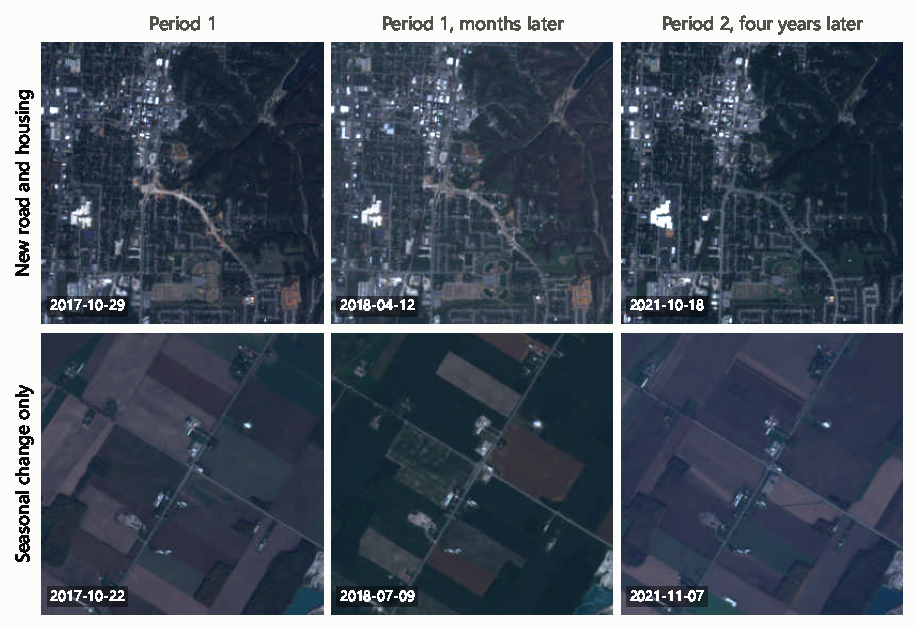
\includegraphics[width=\columnwidth]{pretraining_examples.pdf}
\caption{Two locations from our pretraining data. Top: a road and a new
subdivision are built between the periods. Bottom: fields change colour with the
seasons but not structurally. CACo aims to be invariant to the bottom kind of
change and sensitive to the top kind. Contains modified Copernicus Sentinel data
(2017--2021).}
\label{fig:examples}
\end{figure}

\subsection{Objectives}
All four objectives use the authors' reference implementation~\cite{cacocode}
unchanged; our code wraps it with logging, checkpointing and export. Each
training item yields a query and keys. Negatives come from a per-subspace queue;
SeCo's subspaces 1--2 and all TeCo and CACo subspaces also use other keys in the
batch (MoCo~v2 and SeCo's subspace 0 use only the queue).
\begin{itemize}
\item \textbf{MoCo~v2:} two augmentations of one image, one embedding space. Each
of the 20,000 images is an item.
\item \textbf{SeCo:} three dates of a location drawn from all ten, giving three
subspaces as in~\cite{manas2021seco}. Each location is one item.
\item \textbf{TeCo} (the paper's ``long-term temporal contrast''): the three dates
are drawn, with replacement, from a single period, and the same location's views
from the other period are added as negatives. Each (location, period) pair is an
item.
\item \textbf{CACo:} TeCo with change-awareness; its three dates are drawn
without replacement. For every item, the ratio of the long-term to the
short-term feature distance under the momentum encoder is smoothed with an
exponential moving average (weight 0.8 on history). After every epoch a
two-component Gaussian mixture splits the items into change and no-change; for
no-change items, the long-term key of the same subspace is masked out of the
softmax during the next epoch. Fig.~\ref{fig:hist} shows the estimated ratios.
\end{itemize}

\begin{figure}[t]
\centering
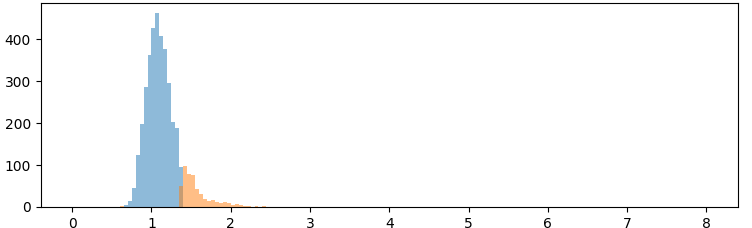
\includegraphics[width=\columnwidth]{change_ratio_histogram.png}
\caption{CACo's change estimates during our pretraining run: histogram of the
smoothed ratio of long-term to short-term feature distance over training items
(x: ratio, y: count). Colours are the two Gaussian-mixture components: no change
(blue) and change (orange).}
\label{fig:hist}
\end{figure}

\subsection{Training}
Every encoder is a ResNet-18 trained on one GPU with SGD (learning rate 0.03,
momentum 0.9, weight decay $10^{-4}$), batch size 256, 128-d embeddings,
temperature 0.07 and encoder momentum 0.999, for 400 epochs with the learning
rate divided by 10 at epochs 250 and 350. Each subspace keeps a queue of 4,096
negatives (the paper uses 16,384). Table~\ref{tab:setup} lists the resulting
optimizer steps and training time, and Fig.~\ref{fig:loss} the loss curves.

\begin{table}[t]
\centering
\caption{Pretraining runs. Steps follow from the dataset items per epoch.}
\label{tab:setup}
\begin{tabular}{lrrrr}
\toprule
 & MoCo & SeCo & TeCo & CACo \\
\midrule
Items per epoch & 20,000 & 2,000 & 4,000 & 4,000 \\
Optimizer steps & 31,200 & 2,800 & 6,000 & 6,000 \\
Training time (GPU-h) & 23.9 & 4.6 & 9.2 & 9.1 \\
\bottomrule
\end{tabular}
\end{table}

\begin{figure*}[t]
\centering
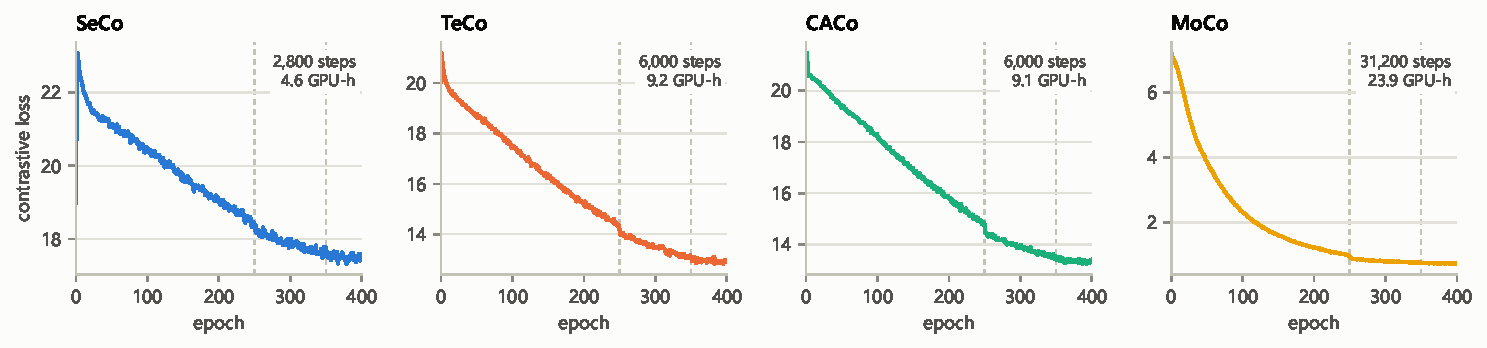
\includegraphics[width=\textwidth]{pretraining_loss.pdf}
\caption{Pretraining loss per epoch. Dashed lines mark the learning-rate drops.
Losses are not comparable across panels because the objectives have different
numbers of subspaces and negatives.}
\label{fig:loss}
\end{figure*}

\subsection{Evaluation}
We evaluate frozen encoders on EuroSAT~\cite{helber2019eurosat} (Sentinel-2,
10 classes, the SeCo/CACo split of 16,200 training and 5,400 test images) and on
UC Merced~\cite{yang2010ucmerced} (aerial imagery at about 0.3\,m per pixel,
21 classes, our stratified split of 1,680/420 images, released with the code).
UC Merced is not used in the paper and differs in sensor and resolution, which
makes it our distribution-shift stress test.

We compare nine encoders: random initialisation, ImageNet~\cite{deng2009imagenet}
weights, our SeCo, TeCo and CACo, and the authors' released 100k MoCo, SeCo,
TeCo and CACo checkpoints. As in the authors' EuroSAT pipeline, images enter as
\texttt{ToTensor()} tensors (UC Merced resized to $256\times256$). Unlike their
probe, which lets BatchNorm statistics adapt during training, we keep the
backbone in evaluation mode so that features are fixed and can be cached. A
linear classifier is trained on the 512-d features with Adam (learning rate
$10^{-3}$) for 100 epochs, decayed by 10 at epochs 60 and 80, batch size 256.
We report final-epoch test accuracy averaged over five probe seeds, plus $k$-NN
($k{=}5$, cosine) accuracy; retrieval precision P@20 is also computed and
released with the code. Differences between
encoders are tested with a paired bootstrap over test images (10,000
resamples)~\cite{efron1993bootstrap}. The intervals resample test images, using
each image's correctness averaged over the five probe seeds; each objective was
pretrained once.

\subsection{Hypotheses}
Before the final evaluation we wrote four hypotheses with decision rules
(released as \texttt{docs/HYPOTHESES.md}). H1, H2 and the released-checkpoint
part of H4 concern models we had not yet evaluated with this protocol; H3 turns
an observation from our first single-seed evaluation into a test.
\begin{itemize}
\item \textbf{H1} (paper Table~6): on EuroSAT, the authors' checkpoints order
SeCo $<$ TeCo $<$ CACo. If the paper's ablation is robust, it should survive a
different probe.
\item \textbf{H2} (paper Table~1): the authors' MoCo~v2 checkpoint is below both
their SeCo and their CACo, since temporal positives add supervision that plain
MoCo~v2 lacks.
\item \textbf{H3} (ablation): at our scale, change-awareness adds less than one
point over TeCo on EuroSAT. With few locations, the change estimates rest on
noisy distance ratios, so the mask may not separate changed from unchanged
places reliably.
\item \textbf{H4} (stress test): ImageNet's lead over the best satellite encoder
of each scale is larger on UC Merced than on EuroSAT, because features tuned to
10\,m Sentinel-2 textures should transfer less well to 0.3\,m aerial imagery
than generic ImageNet features.
\end{itemize}

\section{Results}
Table~\ref{tab:main} lists linear-probe and $k$-NN accuracy for every encoder.
Across five probe seeds the standard deviation is at most 0.17 points on
EuroSAT and 1.03 on UC Merced, so differences between encoders reflect the
features rather than probe randomness.

\begin{table}[t]
\centering
\caption{Frozen-feature accuracy (\%). Linear: final epoch, mean $\pm$ s.d.\ over
five probe seeds. $k$-NN: $k{=}5$, cosine.}
\label{tab:main}
\setlength{\tabcolsep}{4pt}
\begin{tabular}{llcccc}
\toprule
 & & \multicolumn{2}{c}{EuroSAT} & \multicolumn{2}{c}{UC Merced} \\
\cmidrule(lr){3-4}\cmidrule(lr){5-6}
 & Encoder & Linear & $k$-NN & Linear & $k$-NN \\
\midrule
\multirow{2}{*}{--} & Random & 53.00\,$\pm$\,0.13 & 42.98 & 24.14\,$\pm$\,1.03 & 49.29 \\
 & ImageNet & \textbf{87.45}\,$\pm$\,0.04 & 79.74 & \textbf{91.62}\,$\pm$\,0.20 & \textbf{87.86} \\
\midrule
\multirow{3}{*}{\shortstack[l]{Ours\\2k loc.}} & SeCo & 67.42\,$\pm$\,0.05 & 66.31 & 58.24\,$\pm$\,0.80 & 54.76 \\
 & TeCo & 72.23\,$\pm$\,0.06 & 70.37 & 69.05\,$\pm$\,0.41 & 67.14 \\
 & CACo & 72.81\,$\pm$\,0.17 & 70.69 & 67.43\,$\pm$\,0.68 & 67.38 \\
\midrule
\multirow{4}{*}{\shortstack[l]{Authors\\20k loc.}} & MoCo~v2 & 83.37\,$\pm$\,0.03 & 80.48 & 85.76\,$\pm$\,0.39 & 87.14 \\
 & SeCo & 84.32\,$\pm$\,0.04 & 83.69 & 82.95\,$\pm$\,0.49 & 84.29 \\
 & TeCo & 85.77\,$\pm$\,0.06 & 83.63 & 84.19\,$\pm$\,0.27 & 84.76 \\
 & CACo & 86.83\,$\pm$\,0.08 & \textbf{85.09} & 85.19\,$\pm$\,0.35 & 82.62 \\
\bottomrule
\end{tabular}
\end{table}

\subsection{Claim verification}
Table~\ref{tab:claims} tests five quantitative claims. Numbers in the paper come
from its own probing setup, so we compare orderings and gaps, not absolute
values.

\begin{table*}[t]
\centering
\caption{Claims from the paper (ResNet-18) and our tests. Our gaps are paired
differences in linear-probe accuracy with 95\% bootstrap intervals (BigEarthNet:
one run of an MLP probe, micro-averaged average precision, compared as point
estimates). ``Holds'': the paper's direction is reproduced and the interval
excludes zero for every compared model; ``Partly'': this holds for some of them;
``Not reproduced'': for none.}
\label{tab:claims}
\begin{tabular}{p{4.4cm}p{3.9cm}p{6.1cm}l}
\toprule
Claim & Paper & Ours (authors' checkpoints) & Verdict \\
\midrule
CACo improves on SeCo on EuroSAT & 91.42 $\rightarrow$ 93.08, $+1.66$ (Tab.~6)$^a$ & 84.32 $\rightarrow$ 86.83: $+2.51$ $[1.64, 3.39]$ & Holds \\
Long-term contrast, then change-awareness, each add accuracy (H1) & $+1.14$, then $+0.52$ (Tab.~6) & $+1.45$ $[0.59, 2.32]$, then $+1.06$ $[0.26, 1.89]$ & Holds \\
Satellite objectives beat MoCo~v2 on satellite data (H2) & 87.22 $<$ 90.05, 93.08 (Tab.~1)$^b$ & CACo $-$ MoCo $+3.46$ $[2.49, 4.44]$; SeCo $-$ MoCo $+0.94$ $[-0.05, 1.95]$ & Partly \\
Satellite pretraining beats ImageNet on EuroSAT & 86.16 $<$ 93.08 (Tab.~1) & ImageNet $-$ CACo $+0.61$ $[-0.37, 1.61]$ & Not reproduced \\
CACo beats SeCo and ImageNet on BigEarthNet (10\% labels) & 67.89 $>$ 65.80, 65.43 mAP (Tab.~2) & CACo 63.18 $>$ SeCo 60.57; ImageNet 66.17 & Partly \\
\bottomrule
\multicolumn{4}{p{0.95\textwidth}}{\footnotesize $^a$Tab.~6's SeCo with CACo's geographic sampling, which we take to match the released \texttt{\_geo\_} checkpoints; Tab.~1 reports 90.05 $\rightarrow$ 93.08 ($+3.03$) for SeCo with its original sampling.} \\
\multicolumn{4}{p{0.95\textwidth}}{\footnotesize $^b$The released MoCo~v2 checkpoint was trained for 200 epochs; the paper trains its 100k baselines for 1,000.} \\
\end{tabular}
\end{table*}

The paper's component chain reproduces with the released checkpoints: SeCo
$<$ TeCo $<$ CACo on EuroSAT (84.32, 85.77, 86.83), both steps are resolved, and
both intervals contain the paper's increments (Fig.~\ref{fig:steps}). CACo also
beats the authors' MoCo~v2 checkpoint by 3.5 points, but SeCo's lead over it is
not resolved, so H2 is unresolved under its decision rule. Two claims do not
transfer to our probe. ImageNet features are statistically tied with the best
satellite encoder on EuroSAT, and they rank first on BigEarthNet in our earlier
run of a 10\%-label MLP probe (26,969 training patches; 123,648 validation patches
scored), although CACo still beats SeCo there.

\subsection{Ablation at small scale}
Our own pretraining isolates the same two components on one tenth of the data.
Long-term contrast gives a large gain: TeCo beats SeCo by 4.81 points on EuroSAT
and 10.81 on UC Merced (Fig.~\ref{fig:steps}). Change-awareness gives no
detectable gain: CACo $-$ TeCo is $+0.58$ $[-0.28, 1.43]$ on EuroSAT and $-1.62$
$[-5.05, 1.81]$ on UC Merced, so H3 is supported. With the authors' checkpoints
the same step is resolved ($+1.06$). In the reference code CACo also draws its
dates without replacement, so this step measures change-awareness together with
that sampling change, at both scales.

\begin{figure*}[t]
\centering
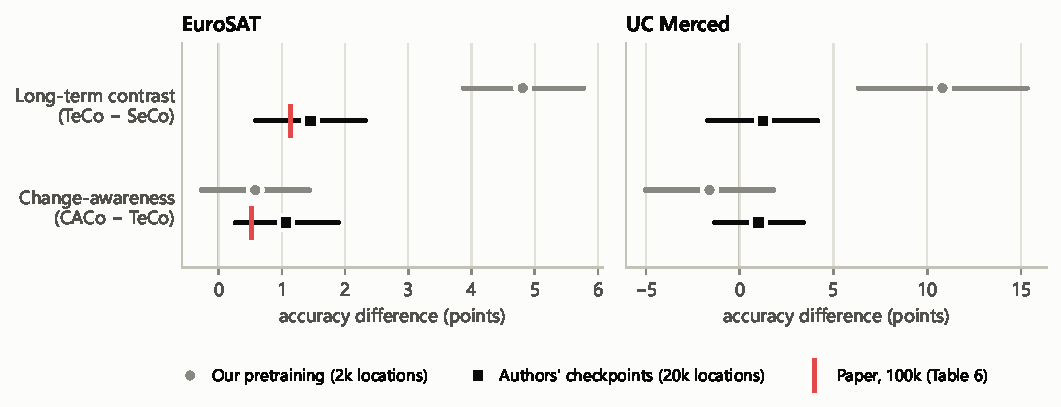
\includegraphics[width=0.82\textwidth]{component_steps.pdf}
\caption{Contribution of each CACo component, as paired accuracy differences with
95\% bootstrap intervals. Red marks are the paper's Table~6 increments (EuroSAT,
100k data).}
\label{fig:steps}
\end{figure*}

Two further observations bear on these comparisons. First, equal epochs are not
equal training: TeCo and CACo see every location once per period, so they take
6,000 optimizer steps against SeCo's 2,800 (Table~\ref{tab:setup}). The released
checkpoints show the same imbalance: their BatchNorm step counters read 156,000
for TeCo and CACo and 78,000 for SeCo (2:1, against 2.1:1 in our runs). Part of the long-term gain at either scale may
therefore come from longer training. Second, our MoCo~v2 encoder, trained under
the same settings but iterating over every image (31,200 steps), scored 79.48\%
on EuroSAT and 84.29\% on UC Merced in our original single-seed evaluation (on
a different UC Merced split from Table~\ref{tab:main}). That beats all three
temporal objectives at our scale. With the released checkpoints, where MoCo~v2
had a comparable number of steps (156,200), CACo is ahead on EuroSAT ($+3.46$)
and level with it on UC Merced ($-0.57$ $[-3.33, 2.24]$). Training length, not
just the objective, has to be controlled when comparing these methods.

\subsection{Stress test: UC Merced}
UC Merced images have about 30 times finer resolution than Sentinel-2, a regime
the paper names as a limitation. As predicted (H4), ImageNet's lead over the
best satellite encoder grows on it: from 0.6 to 5.9 points for the released
checkpoints, where MoCo~v2 is the best satellite encoder on UC Merced (85.76\%),
and from 14.6 to 22.6 points over our best temporal encoder. Our MoCo~v2
encoder, measured only in the original single-seed evaluation, does not follow
this pattern: ImageNet's lead over it falls from 8.0 to 5.7 points. The released
temporal checkpoints keep their EuroSAT ordering on UC Merced, but neither step
is resolved ($+1.24$ and $+1.00$); at our scale CACo falls slightly below TeCo
($-1.62$, within noise). Fig.~\ref{fig:failures} shows test images that ImageNet
features classify correctly and the CACo checkpoint does not. Some of these
errors are between related classes (dense vs.\ medium residential, chaparral
vs.\ forest); others confuse distinct objects (storage tanks, parking lots and
intersections predicted as airplanes).

\begin{figure}[t]
\centering
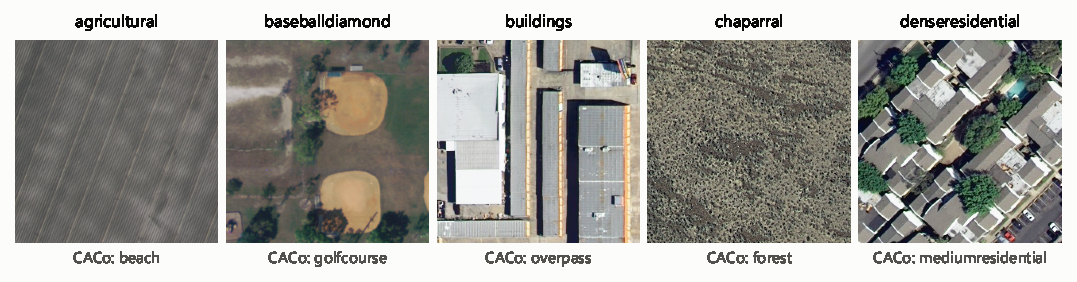
\includegraphics[width=\columnwidth]{failure_examples.pdf}
\caption{UC Merced test images classified correctly from ImageNet features but
misclassified from the authors' CACo checkpoint in every probe seed (37 of 420).
Titles: true class; below: CACo's prediction.}
\label{fig:failures}
\end{figure}

\subsection{What the paper doesn't tell you}
\textbf{The probe protocol moves the numbers.} Table~\ref{tab:protocol} probes the
same released checkpoints in two ways. With ImageNet-normalized inputs,
BatchNorm statistics that adapt during probe training and batch size 64, CACo
(93.31\%) and random initialisation (62.80\%) come close to the paper's 93.08\%
and 64.21\%, while SeCo (93.06\%) exceeds the paper's SeCo. With a frozen
backbone and raw inputs, random initialisation drops by almost ten points and
the pretrained satellite encoders by 6.5 to 8.7, and ImageNet moves from below
both satellite encoders to above them (its lead over CACo is within noise). The
CACo $-$ SeCo gap is $+0.25$ under one protocol and $+2.51$ under the other,
against $+1.66$ in the paper. The encoders were pretrained on ImageNet-normalized
inputs, so feeding raw inputs to a frozen backbone shifts its input
distribution; re-estimating BatchNorm statistics is one way to absorb that
shift. Comparisons across papers are only meaningful under one protocol.

\begin{table}[t]
\centering
\caption{EuroSAT accuracy of the same encoders under two probe protocols.
BN-adapt: ImageNet-normalized inputs, BatchNorm statistics updated during probe
training, batch 64, final epoch, one seed. Frozen: Table~\ref{tab:main}.}
\label{tab:protocol}
\begin{tabular}{lccc}
\toprule
Encoder & Paper & BN-adapt & Frozen \\
\midrule
Random & 64.21 & 62.80 & 53.00 \\
ImageNet & 86.16 & 85.26 & 87.45 \\
SeCo 100k & 91.42$^\dagger$ & 93.06 & 84.32 \\
CACo 100k & 93.08 & 93.31 & 86.83 \\
\midrule
CACo $-$ SeCo & $+1.66$ & $+0.25$ & $+2.51$ \\
\bottomrule
\multicolumn{4}{l}{\footnotesize $^\dagger$Tab.~6 (SeCo with CACo's sampling); Tab.~1 lists 90.05.} \\
\end{tabular}
\end{table}

\textbf{SeCo gets half the training.} The paper notes that TeCo and CACo batches
hold half as many locations, but it does not report that this doubles their
optimizer steps relative to SeCo, or control for it. Our runs (2.1:1) and the released
checkpoints (2:1) both show this imbalance, so the paper's long-term-contrast
increment mixes a new objective with longer training.

\textbf{The change mask is partial.} In the reference code, an item judged
unchanged loses one long-term key per subspace: the key from that subspace. In
subspace 0 this is its only long-term negative, but in the other two subspaces
the other subspaces' keys for the other period remain negatives. Together with
the sampling difference above, CACo and TeCo differ in two ways, and the mask is
narrower than the paper's description suggests. In our run the ratio
distribution is unimodal with a right tail (Fig.~\ref{fig:hist}); the mixture
model labels the tail as changed, so most items are treated as unchanged.

\textbf{``10k'' and ``100k'' appear to count images per period.} The public 10k
archive holds 2,000 locations with five images per period, and the released
100k checkpoints imply 20,000 locations.

\section{Challenges}
\textbf{Compute.} Each pretraining run used one cluster GPU: 4.6 hours for SeCo,
about 9 for TeCo and CACo, and 23.9 for MoCo~v2, which iterates over all 20,000
images every epoch. Because the reference code pins PyTorch~1.7 and PyTorch
Lightning~1.1.8, we kept a separate legacy environment for training and ran all
evaluation in a current one.

\textbf{Weak training signal.} The four losses are not comparable with one
another (Fig.~\ref{fig:loss}), so the only way to know whether a run had worked
was to probe it downstream. We therefore built a feature-caching probe harness
that re-evaluates an encoder in about two minutes on a laptop CPU.

\textbf{Data access.} The original download links for BigEarthNet and UC Merced
no longer resolve. We used the official Zenodo release of
BigEarthNet~\cite{sumbul2019bigearthnet} and the TorchGeo~\cite{stewart2022torchgeo}
mirror of UC Merced, and we release our UC Merced split.

\textbf{Inconsistent early numbers.} Our first EuroSAT probes, run on Colab and on
the cluster, gave the same randomly initialised network 62.8\% and 53.1\%.
Tracing this to the probe protocol (Table~\ref{tab:protocol}) led us to evaluate
every encoder with a single harness, five seeds and paired tests.

\section{Ethics}
\textbf{Surveillance.} Our pretraining uses Sentinel-2 imagery at 10\,m per pixel,
where people, vehicles and most individual houses are not resolvable; the UC Merced
stress test uses public 0.3\,m aerial imagery of land-use scenes.
Representations trained to notice change could still be applied to
higher-resolution imagery to monitor properties, movements or gatherings, and
that use deserves oversight.

\textbf{Geographic bias.} The pretraining locations are sampled around the world's
most populated cities. The features are therefore tuned to urban growth and
temperate agriculture, and may serve informal settlements, smallholder farms or
arid and polar regions poorly. These are often the places where remote sensing
could help most.

\textbf{Compute.} Our four pretraining runs logged 46.8 GPU-hours. The main
evaluation (Table~\ref{tab:main}) ran on a laptop CPU in under an hour by
caching features.

\section{Reflection}
\textbf{Overall.} The project delivered what we set out to test: the paper's
ablation reproduces with its released checkpoints, while at small scale the
change-awareness component shows no measurable effect.

\textbf{Goals.} Our base goal was to pretrain SeCo and CACo with the reference code
and show they beat random initialisation; we did, by 14 to 20 points on
EuroSAT. Our target goal was a controlled ablation of CACo's components (TeCo)
and a check of the paper's claims against its checkpoints; we did both. Our
stretch goal, a distribution-shift test on a dataset the paper does not use,
became the UC Merced evaluation.

\textbf{Did it work as expected?} Partly. We expected change-awareness to matter
most when data is scarce; instead it was undetectable at our scale and resolved
only with the authors' checkpoints, which used ten times more locations and
longer training. We did not expect plain MoCo~v2 or ImageNet features to be so
competitive, or the probe protocol to move results as much as the choice of
objective.

\textbf{How the project evolved.} We began by trying to match the paper's
numbers. When our first evaluations disagreed with each other, we shifted to
controlled comparisons: one harness for all encoders, several probe seeds,
paired tests, and hypotheses written down before the final evaluation. If we
started over, we would fix the evaluation protocol first, log optimizer steps for
every objective, and save per-image predictions from the very first run.

\textbf{With more time} we would match optimizer steps across objectives, add
pretraining seeds to measure run-to-run variance, evaluate change detection on
OSCD, where CACo reports its largest gains, and try a soft change mask using
the mixture posterior.

\textbf{Takeaways.} Controls matter as much as models: equal epochs are not equal
compute, and evaluation protocol can outweigh architectural choices. Strong
simple baselines (MoCo~v2, ImageNet) belong in every table. Ablations should
ask what each component buys, not just whether the full method wins.

\section*{Acknowledgments}
We thank Professor Randall Balestriero and our mentor TA Daniel Zhu for their
guidance, the CSCI~1470 course staff, and Mall, Hariharan and Bala for releasing
their code, data and checkpoints; their code builds on the SeCo
codebase~\cite{secocode}. Pretraining used Brown University's Center for
Computation and Visualization (CCV). Software: PyTorch and
torchvision~\cite{paszke2019pytorch}, PyTorch Lightning~\cite{falcon2019lightning},
scikit-learn~\cite{pedregosa2011sklearn}, NumPy~\cite{harris2020numpy},
SciPy~\cite{virtanen2020scipy}, pandas~\cite{mckinney2010pandas} and
Matplotlib~\cite{hunter2007matplotlib}; UC Merced via the
TorchGeo~\cite{stewart2022torchgeo} mirror.

\bibliographystyle{IEEEtran}
\bibliography{references}

\end{document}
